\documentclass[12pt]{article}
\usepackage[utf8]{inputenc}
\usepackage[russian]{babel}
\usepackage{graphicx}
\usepackage{array}
\usepackage[a4paper, left=1cm, right=1cm, top=1.27cm, bottom=1.27cm]{geometry}
\usepackage{setspace}
\usepackage{tabularx}
\usepackage{makecell}
\usepackage{longtable}
\usepackage{multirow}
\usepackage{caption}
\onehalfspacing


\begin{document}


\begin{table}[h]
    \centering
    \renewcommand{\arraystretch}{1.5} % Увеличиваем межстрочный интервал
    \begin{tabular}{|m{11cm}|m{6cm}|} % Первая колонка шире, вторая для лого
        \hline
        \begin{center}
            \textbf{Университет ITMO}\\
            \textbf{Физико-технический мегафакультет}\\
            \textbf{Физический факультет}
        \end{center} 
        & 
        \begin{center}
            
\includegraphics[height=1.3cm]{logo.jpg}
        \end{center} \\
        \hline
    \end{tabular}
\end{table}

\noindent\makebox[\linewidth]{\rule{\textwidth}{2pt}}

\vspace{10pt}

\begin{table}[h]
    \centering
    \renewcommand{\arraystretch}{1.7}
    \begin{tabular}{|p{4cm}p{4cm}|p{8cm}|}
        \hline
        Группа N3150 & & К работе допущен \underline{\hspace{4cm}} \\
        \hline
        Студенты & \hfill \multirow[0pt]{3}{*}{\makecell[c]{Пахомов В.Ю \\ Фармахини Ф.Р. \\ Петров Д.О}}  & Работа выполнена \underline{\hspace{4cm}} \\
        & & \\
        & & \\
        \hline
        \multicolumn{2}{|c|}{Преподаватель \underline{\hspace{5cm}}}  & Отчет принят \underline{\hspace{5cm}} \\
        \hline
    \end{tabular}
\end{table}

\begin{center}
    \fontsize{20pt}{21.5pt} \selectfont
    \textbf{Рабочий протокол и отчет по}\\
    \textbf{лабораторной работе № 1.04}
\end{center}

\noindent\makebox[\linewidth]{\rule{\textwidth}{1pt}}
\noindent\makebox[\linewidth]{\rule{\textwidth}{1pt}}

\begin{flushleft}
    1. Цель работы.\\
    \hspace{0.63cm}1) Проврека основного закона динамики вращения. \\
    \hspace{0.63cm}2) Проверка зависимости момента инерции от
    положения масс относительно оси вращения.

\end{flushleft}

\begin{flushleft}
    2. Задачи, решаемые при выполнении работы.\\
    \hspace{0.63cm} 1) Измерение времени падения груза при разной массе груза и разном положении утяжелителей на крестовине. \\
    \hspace{0.63cm} 2) Расчёт ускорения груза, углового ускорения крестовины и момента силы натяжения нити. \\
    \hspace{0.63cm} 3) Расчёт момента инерции крестовины с утяжелителями и момента силы трения. \\
    \hspace{0.63cm} 4) Исследование зависимости момента силы натяжения нити от углового ускорения. Проверка основного закона динамики вращения. \\
    \hspace{0.63cm} 5) Исследование зависимости момента инерции от положения масс относительно оси вращения. Проверка теоремы Штейнера. \\
\end{flushleft}

\begin{flushleft}
    3. Объект исследования. \\
    Динамика вращательного движения крестовины с утяжелителями
    при воздействии силы натяжения нити, создаваемой падающим грузом. \\
\end{flushleft}

\begin{flushleft}
    4. Метод экспериментального исследования. \\
    Экспериментальный метод с прямыми измерениями кинематических параметров движения 
    груза и крестовины. Измеряется время движения груза, вычисляются его ускорение, 
    угловое ускорение крестовины и момент силы натяжения нити. На основе метода
    наименьших квадратов (МНК) определяются момент инерции крестовины и момент
    силы трения. \\

\end{flushleft}

\begin{flushleft}
    5. Рабочие формулы и исходные данные. \\
\end{flushleft}

\newpage

\begin{flushleft}
    6. Измерительные приборы.
\end{flushleft}

\begin{table}[h]
    \centering
    \renewcommand{\arraystretch}{1.5}
    {\itshape
    \begin{tabular}{|c|c|c|c|c|}
        \hline
        № п/п & Наименование & Тип прибора & Используемый диапазон & Погрешность прибора\\
        \hline
        1 & Секундомер & Электронный & 0-60 с & ±0.01 с \\
        \hline
        2 & Линейка & Металлическая & 0-700 мм с & ±0.5 мм \\
        \hline
    \end{tabular}
    }
\end{table}

\begin{flushleft}
    7. Схема установки. \\
    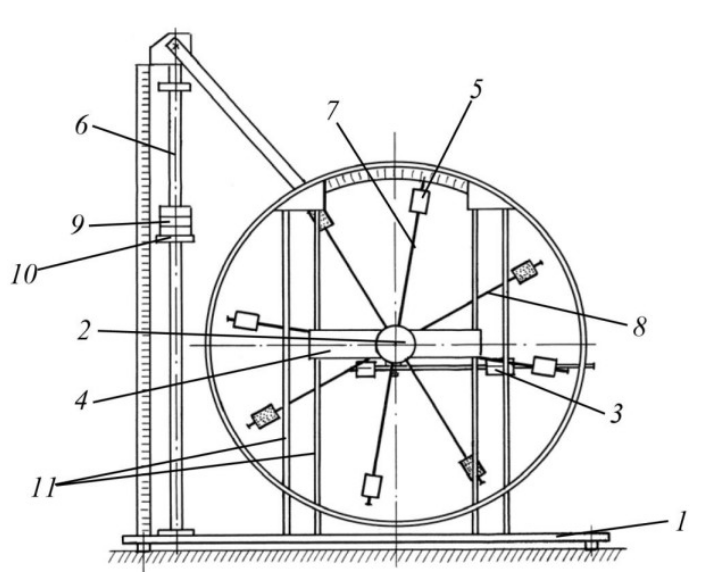
\includegraphics[height=10cm]{schema.png} \\
    В состав установки входят: \\
    \hspace{0.63cm}1. Основание \\
    \hspace{0.63cm}2. Рукоятка сцепления крестовин \\
    \hspace{0.63cm}3. Устройства принудительного трения \\
    \hspace{0.63cm}4. Поперечина \\
    \hspace{0.63cm}5. Груз крестовины \\
    \hspace{0.63cm}6. Трубчатая направляющая \\
    \hspace{0.63cm}7. Передняя крестовина \\
    \hspace{0.63cm}8. Задняя крестовина \\
    \hspace{0.63cm}9. Шайбы каретки \\
    \hspace{0.63cm}10. Каретка \\
    \hspace{0.63cm}11. Система передних стоек \\
\end{flushleft}

\begin{flushleft}
    8. Результаты прямых измерений и их обработки. \\
\end{flushleft}
\begin{table}[h]
    \centering
    \renewcommand{\arraystretch}{1.3}
    \setlength{\tabcolsep}{8pt}
    \captionsetup{justification=centering, font=bf}
    \caption{Протокол измерений времени падения груза при разной массе груза и разном положении утяжелителей на крестовине}
    \begin{tabular}{|c|c|c|c|c|c|c|}
        \hline
        Масса & \multicolumn{6}{c|}{Положение утяжелителей} \\
        \cline{2-7}
        груза, г & 1 риска & 2 риска & 3 риска & 4 риска & 5 риска & 6 риска \\
        \hline
        \multirow{4}{*}{$m_1$} & $t_1$ 4.62 & 5.37 & 6.13 & 7.04 & 7.87 & 9.12 \\
        \cline{2-7}
        & $t_2$ 4.51 & 5.29 & 6.24 & 7.21 & 7.73 & 9.12 \\
        \cline{2-7}
        & $t_3$ 4.69 & 5.30 & 6.10 & 6.98 & 7.81 & 9.05 \\
        \cline{2-7}
        & $t_{cp}$ 4.61 & 5.32 & 6.16 & 7.07 & 7.80 & 9.10 \\
        \hline
        \multirow{4}{*}{$m_2$} & 3.71 & 4.31 & 5.10 & 5.31 & 6.00 & 6.75 \\
        \cline{2-7}
        & 3.7 & 4.43 & 5.37 & 5.30 & 5.89 & 6.83 \\
        \cline{2-7}
        & 3.68 & 4.36 & 5.21 & 5.26 & 6.13 & 6.80 \\
        \cline{2-7}
        & 3.70 & 4.37 & 5.23 & 5.31 & 6.01 & 6.80 \\
        \hline
        \multirow{4}{*}{$m_3$} & 2.91 & 3.67 & 4.14 & 4.59 & 5.09 & 5.66 \\
        \cline{2-7}
        & 3.13 & 3.61 & 4.27 & 4.51 & 5.15 & 5.64 \\
        \cline{2-7}
        & 3.13 & 3.55 & 4.34 & 4.54 & 4.8 & 5.65 \\
        \cline{2-7}
        & 3.06 & 3.61 & 4.25 & 4.55 & 5.01 & 5.65 \\
        \hline
        \multirow{4}{*}{$m_4$} & 2.79 & 3.22 & 3.52 & 4.02 & 4.34 & 5.00 \\
        \cline{2-7}
        & 2.71 & 3.14 & 3.42 & 3.98 & 4.37 & 5.10 \\
        \cline{2-7}
        & 2.78 & 3.27 & 3.51 & 3.85 & 4.32 & 5.13 \\
        \cline{2-7}
        & 2.76 & 3.21 & 3.48 & 3.95 & 4.34 & 5.08 \\
        \hline
    \end{tabular}
\end{table}


\newpage


\begin{flushleft}
    9. Расчет результатов косвенных измерений (таблицы, примеры расчетов). \\
    Линейное ускорение: $ \alpha = \frac{2h}{t^2} $ \\
    Угловое ускорение: $ \epsilon = \frac{2\alpha}{d} $ \\
    Момент силы натяжения: $ M = \frac{md}{2}(g - \alpha) $ \\
\end{flushleft}

\begin{table}[h]
    \centering
    \renewcommand{\arraystretch}{1.3}
    \setlength{\tabcolsep}{8pt}
    \captionsetup{justification=centering, font=bf}
    \caption{Рассчёты линейного и углового ускорений груза и момент силы натяжения}
    \begin{tabular}{|c|c|c|c|c|}
        \hline
        Масса груза, г & Риски & Уск. $ a $ & Уск. $ \epsilon $ & Момент $ M $ \\
        \hline
        \multirow{6}{*}{$m_1$} & 1 риска & 0.066 & 2.86 & 0.04928 \\
        \cline{2-5}
        & 2 риска & 0.049 & 2.15 & 0.04939 \\
        \cline{2-5}
        & 3 риска & 0.037 & 1.60 & 0.04950 \\
        \cline{2-5}
        & 4 риска & 0.028 & 1.22 & 0.04950 \\
        \cline{2-5}
        & 5 рисок & 0.023 & 1.00 & 0.04950 \\
        \cline{2-5}
        & 6 рисок & 0.017 & 0.74 & 0.04950 \\
        \hline
        \multirow{6}{*}{$m_2$} & 1 риска & 0.102 & 4.45 & 0.09823 \\
        \cline{2-5}
        & 2 риска & 0.073 & 3.19 & 0.09856 \\
        \cline{2-5}
        & 3 риска & 0.051 & 2.23 & 0.09878 \\
        \cline{2-5}
        & 4 риска & 0.050 & 2.16 & 0.09878 \\
        \cline{2-5}
        & 5 рисок & 0.039 & 1.69 & 0.09889 \\
        \cline{2-5}
        & 6 рисок & 0.030 & 1.32 & 0.09900 \\
        \hline
        \multirow{6}{*}{$m_3$} & 1 риска & 0.150 & 6.50 & 0.14663 \\
        \cline{2-5}
        & 2 риска & 0.107 & 4.67 & 0.14729 \\
        \cline{2-5}
        & 3 риска & 0.078 & 3.37 & 0.14773 \\
        \cline{2-5}
        & 4 риска & 0.068 & 2.94 & 0.14784 \\
        \cline{2-5}
        & 5 рисок & 0.056 & 2.43 & 0.14806 \\
        \cline{2-5}
        & 6 рисок & 0.044 & 1.91 & 0.14828 \\
        \hline
        \multirow{6}{*}{$m_4$} & 1 риска & 0.184 & 7.99 & 0.19481 \\
        \cline{2-5}
        & 2 риска & 0.136 & 5.91 & 0.19580 \\
        \cline{2-5}
        & 3 риска & 0.116 & 5.03 & 0.19624 \\
        \cline{2-5}
        & 4 риска & 0.090 & 3.90 & 0.19679 \\
        \cline{2-5}
        & 5 рисок & 0.074 & 3.23 & 0.19701 \\
        \cline{2-5}
        & 6 рисок & 0.054 & 2.36 & 0.19745 \\
        \hline
    \end{tabular}
\end{table}


\newpage


\begin{table}[h]
    \centering
    \renewcommand{\arraystretch}{1.3}
    \setlength{\tabcolsep}{8pt}
    \captionsetup{justification=centering, font=bf}
    \caption{Рассчёт $ M_{tr} $ и $ I $ методом наименьших квадратов}
    \begin{tabular}{|c|c|c|}
        \hline
        & $ M_{tr} $ & $ I $ \\
        \hline
        1 риска & -0.0268102 & 0.0272106 \\
        \hline
        2 риска & -0.0263766 & 0.0389390 \\
        \hline
        3 риска & -0.0034378 & 0.0410382 \\
        \hline
        4 риска & -0.0187718 & 0.0555770 \\
        \hline
        5 риска & -0.0146202 & 0.0661007 \\
        \hline
        6 риска & -0.0191277 & 0.0901644 \\
        \hline

    \end{tabular}
\end{table}

\begin{table}[h]
    \centering
    \renewcommand{\arraystretch}{1.3}
    \setlength{\tabcolsep}{8pt}
    \captionsetup{justification=centering, font=bf}
    \caption{Рассчёт $ R, R^2 $} 
    \begin{tabular}{|c|c|c|}
        \hline
        $ R $ & $ R^2 $ & $ I $ \\
        \hline
        0.077	&	0.005929	&	0.0272106 \\
        \hline
        0.102	&	0.010404	&	0.0389390 \\
        \hline
        0.127	&	0.016129	&	0.0410382 \\
        \hline
        0.152	&	0.023104	&	0.0555770 \\
        \hline
        0.177	&	0.031329	&	0.0661007 \\
        \hline
        0.202	&	0.040804	&	0.0901644 \\
        \hline

    \end{tabular}
\end{table}


\begin{flushleft}
    10. Расчет погрешностей измерений (для прямых и косвенных измерений). \\
    $ h = 700 \pm 0.5 $ мм \\
    $ d = 46 \pm 0.5 $ мм \\
    $ m = 220 \pm 0.5 $ г \\
    Расчет погрешности $ \Delta t $ для первого значения: \\ 
    Cреднеквадратичное отклонение среднего значения: $ \sigma_{\langle t \rangle} = \sqrt{\frac{1}{N - 1} \sum_{i=1}^{N} (t_i - \langle t \rangle_N)^2} \approx 0.091 $ \\
    Погрешность среднего значения: $ \Delta t = \frac{\sigma_t}{\sqrt{N}} = \frac{0.091}{\sqrt{3}} \approx 0.052 $ c \\
    Рассчёт погрешностей для первых $ \alpha, \epsilon, M $: \\
    $ \Delta \alpha = \alpha\sqrt{(\frac{\Delta h}{h})^2 + (2\frac{\Delta t}{t})^2} = 0.066 \pm 0.0015 $ \\
    $ \Delta \epsilon = \epsilon\sqrt{(\frac{\Delta \alpha}{\alpha})^2 + (\frac{\Delta d}{d})^2} = 2.86 \pm 0.072$ \\
    $ \Delta M = M\sqrt{(\frac{\Delta d}{d})^2 + (\frac{\Delta \alpha}{g - \alpha})^2} = 0.04928 \pm 0.00054 $ \\
    $ I_0 \approx 0.0169 \pm 0.0033 $ \\
    $ m_{yt} \approx 0.4255 \pm 0.034 $ \\
\end{flushleft}

\newpage

\begin{flushleft}
    11. Графики (перечень графиков, которые составляют Приложение 2). \\
\end{flushleft}

\begin{flushleft}
    График зависимости $ I(R^2) $: \\
    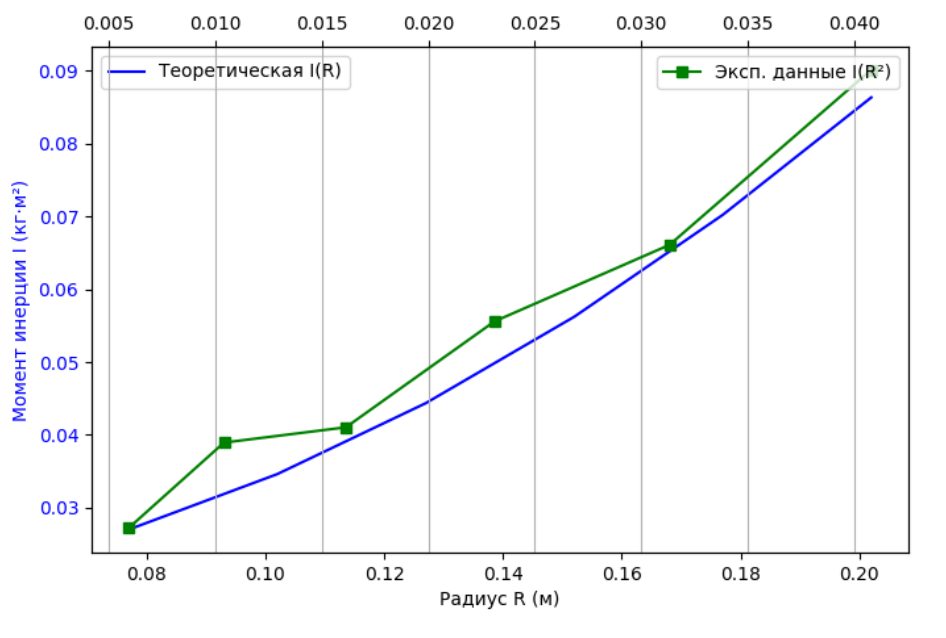
\includegraphics[height=9cm]{chart_IR2.png}
\end{flushleft}

\begin{flushleft}
    График зависимости $ M(\epsilon) $: \\
    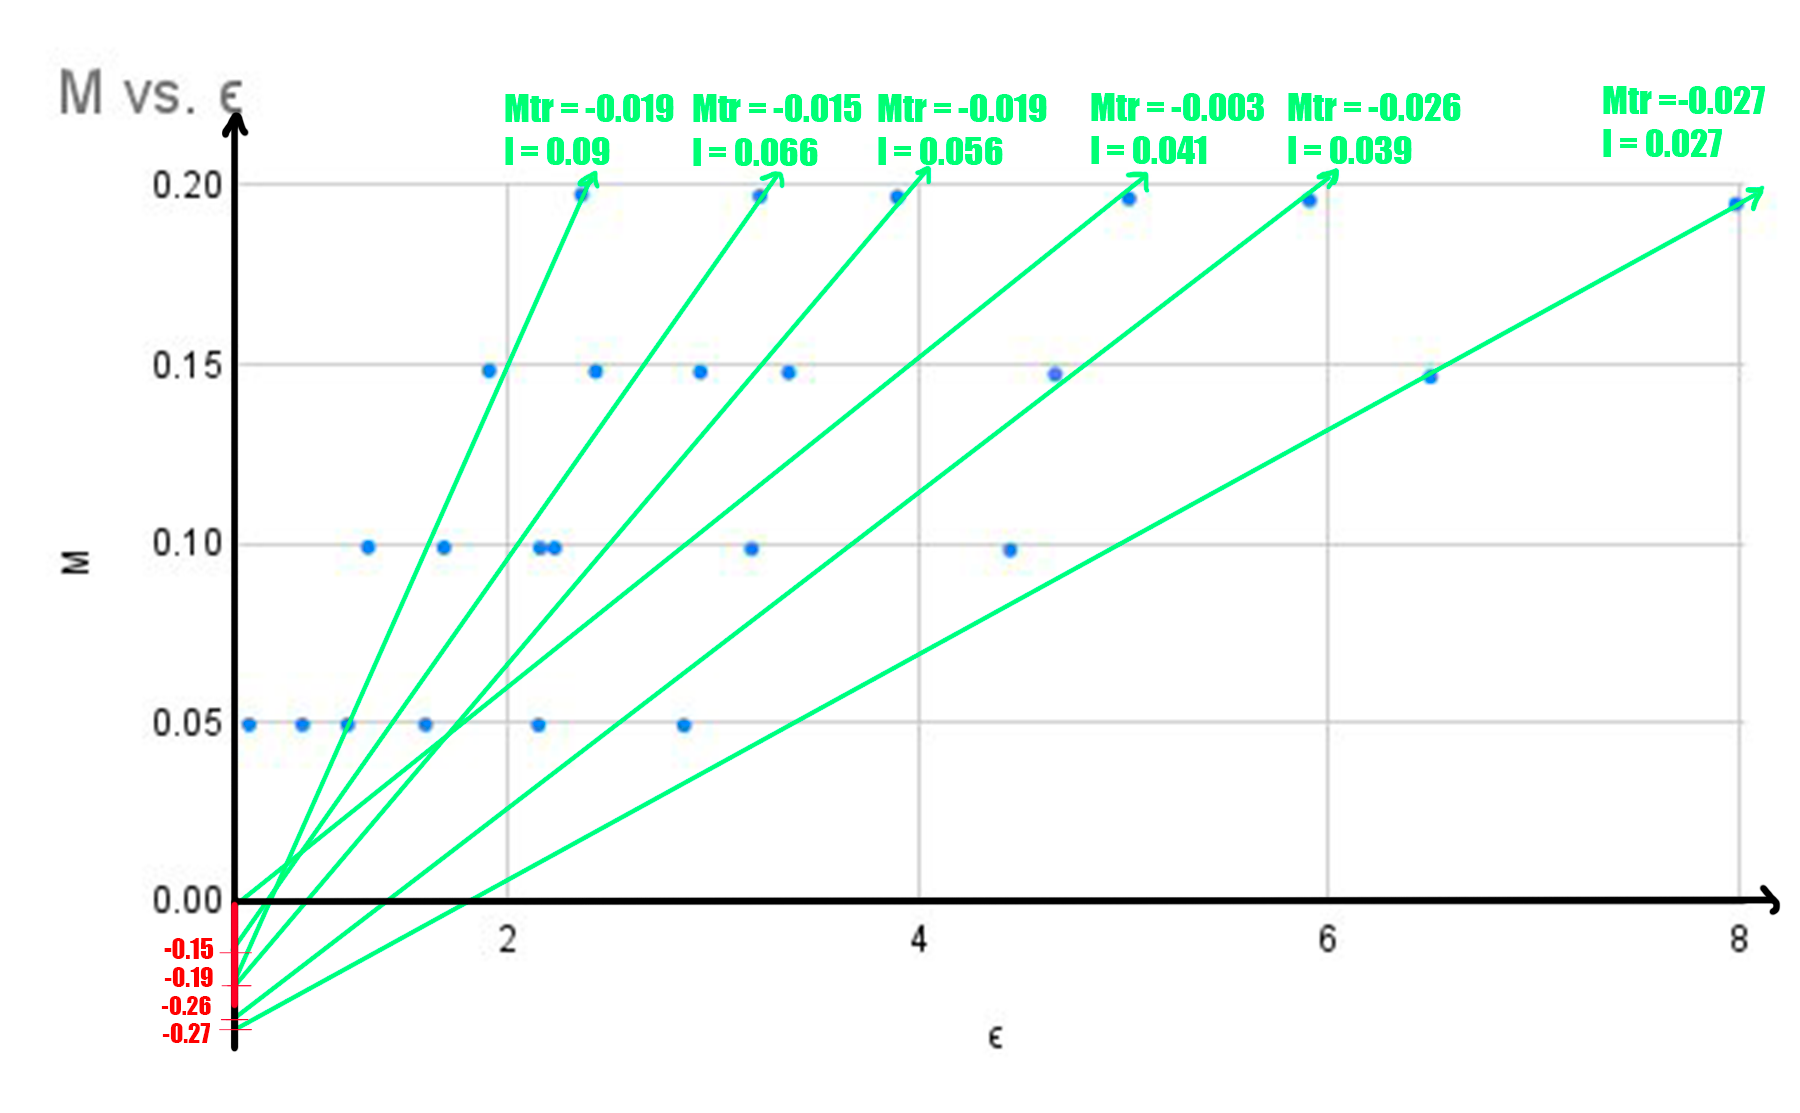
\includegraphics[height=8cm]{chart2.png}
\end{flushleft}


\begin{flushleft}
    12. Окончательные результаты. \\
    $ I_0 = 0.0169 \pm 0.0033 $ \\
    $ m_{yt} = 0.4255 \pm 0.034 $ \\
    $ \Delta t = 0.052 $ c \\
    $ \Delta \alpha = 0.066 \pm 0.0015 $ \\
    $ \Delta \epsilon = 2.86 \pm 0.072$ \\
    $ \Delta M = 0.04928 \pm 0.00054 $ \\

\end{flushleft}

\begin{flushleft}
    13. Выводы и анализ результатов работы. \\
    Зависимость момента силы натяжения нити $ (M) $ от углового ускорения $ (\epsilon) $ для всех положений утяжелителей оказалась линейной. Коэффициенты корреляции близки к 1, что подтверждает справедливость уравнения $ M = M_{tr} + I \epsilon $. \\
    Момент инерции $ I $ возрастал с увеличением $ R^2 $ (квадрата расстояния утяжелителей от оси). Экспериментальные точки легли на прямую, описываемую формулой $ I = I_0 + 4m_{yt}R^2 $, что согласуется с теоремой Штейнера. \\
    Основной закон динамики вращения ($ M - M_{tr} = I \epsilon $) подтверждён: линейная зависимость $ M(\epsilon) $ и соответствие расчётных $ I $ экспериментальным данным. \\
    Зависимость момента инерции от положения масс $ I \approx R^2 $ подтверждает теорему Штейнера. \\
    Погрешности связаны с неточностями измерения времени, силой трения в оси крестовины и возможным проскальзыванием нити. \\
\end{flushleft}

\begin{flushleft}
    14. Дополнительные задания. \\
\end{flushleft}

\begin{flushleft}
    15. Выполнение дополнительных заданий. \\
\end{flushleft}

\begin{flushleft}
    16. Замечания преподавателя (исправления, вызванные замечаниями преподавателя, также помещают в этот пункт). \\
\end{flushleft}

\end{document}